\documentclass[
	%parspace, % Add vertical space between paragraphs
	%noindent, % No indentation of first lines in each paragraph
	%nohyp, % No hyphenation of words
	%twoside, % Double sided format
	%draft, % Quicker draft compilation without rendering images
	%final, % Set final to hide todos
]{elteikthesis}[2024/04/26]

% \pdfobjcompresslevel=0 % Disable object compression

% The minted package is also supported for source highlighting
% See elteikthesis_minted.tex for example
%\usepackage[newfloat]{minted}

% Document's metadata
\title{LiDAR-Based Mapping Module\\For Autonomous Navigation } % title
\date{2025} % year of defense

% Author's metadata
\author{Zewdie-Habtie Sisay}
\degreetitle{MSc Intelligent Field Robotic Systems (IFRoS)}

% Superivsor(s)' metadata
\supervisor{Zoltán Istenes} % internal supervisor's name
\affiliation{Professor} % internal supervisor's affiliation
\extsupervisor{Mohammad Albaja} % external supervisor's name
\extaffiliation{Associate Professor, SMART } % external supervisor's affiliation

% University's metadata
\university{Eötvös Loránd University} % university's name
\faculty{Faculty of Informatics} % faculty's name
\department{Erasmus Mundus Joint Master in \\Intelligent Field Robotic Systems} % department's name
\city{Budapest} % city
\logo{elte_cimer_szines} % logo

% Add bibliography file
\addbibresource{bibliography.bib}
%
\makeglossaries

\newglossaryentry{surveying}
{
    name=surveying,
    description={The work of examining and recording the area and features of a piece of land in order to construct a map, plan, or detailed description thereof}
}

\newglossaryentry{pointcloud}
{
    name={point cloud},
    description={A set of point coordinates obtained as the output of a scanning sensor}
}

\newglossaryentry{fieldrob}
{
    name={Field Robotics},
    description={The area of robotics that focuses on robots operating in unstructured outdoor environments for tasks like agriculture or exploration}
}

\newglossaryentry{registration}
{
    name={registration},
    description={The process of aligning multiple point clouds in a single coordinate system such that matching features are as close as possible}
}

\newglossaryentry{odometry}
{
name={odometry},
    description={The process of computing relative displacement of a robot using on-board sensors}
}

\newglossaryentry{sfm}{
    name={Structure from Motion (SfM)},
    description={The task of reconstructing a 3D scene and a sequence of camera poses from a set of images}
}

\newglossaryentry{kdtree}{
    name={k-d tree},
    description={A data structure for organizing entries in a $k$-dimensional space using a tree structure. When $k$ is not very large, it provides logarithmic look-up time.}
}

\newglossaryentry{voxel}{
    name={voxel},
    description={A cuboid-shaped region in 3D space; a 3D cell.}
}

\newglossaryentry{keyframe}{
    name={keyframe},
    description={An image frame or 3D scan that is used for odometry estimation. Because modern sensors usually operate at higher frequencies than needed for most algorithms, it is a reasonable decision to skip frames based on a predefined pattern or condition, without sacrificing accuracy.}
}

\newacronym{lidar}{LiDAR}{Light Detection and Ranging}
\newacronym{slam}{SLAM}{Simultaneous Localization and Mapping}
\newacronym{ins}{INS}{Inertial Navigation System}
\newacronym{gnss}{GNSS}{Global Navigation Satellite System}
\newacronym{rtk}{RTK}{Real-Time Kinematics}
\newacronym{kf}{KF}{Kalman Filter}
\newacronym{ekf}{EKF}{Extended Kalman Filter}
\newacronym{pf}{PF}{Particle Filter}
\newacronym{icp}{ICP}{Iterative Closest Point}
\newacronym{ndt}{NDT}{Normal Distributions Transform}
\newacronym{loam}{LOAM}{LiDAR Odometry and Mapping}
\newacronym{lio}{LIO}{LiDAR-Inertial Odometry}
\newacronym{cnn}{CNN}{Convolutional Neural Network}



% The document
\begin{document}

% Set document language
\documentlang{english}

% List of todos (not in the final document)
%\listoftodos[\todolabel]

% Custom commands

\newcommand{\reffig}[1]{(Fig. \ref{fig:#1})}
\newcommand{\refch}[1]{(Chapter \ref{ch:#1})}



% Title page (mandatory)
\maketitle
% Topic declaration page (mandatory) - can also be attached instead

\includepdf[pages={2,3}]{other/Z_signed.pdf}

% Table of contents (mandatory)
\tableofcontents
\cleardoublepage

% Main content
\chapter{Introduction}
\label{ch:intro}

% - General description of robotics;
% - General description of perception;
% - General description of localization.

Like many scientific terms that we encounter in our daily activities, \emph{robotics} describes a broad collection of technologies and stands at the intersection of key research directions. Motivated by practicality, disciplines that appear completely unrelated find themselves building upon advancements in other fields, diluting boundaries and joining forces to enable otherwise-impossible advancements.

What constitutes a \emph{robot}, then? In its inceptive use by Karel Čapek \cite{roberts_robotics_history_1999} in 1921, the word stemmed from the Slavic \emph{robota}, meaning ``servitude'' or ``forced work'', and referred to a human-like mechanical system working on factory assembly lines. This concept, however, dates from earlier centuries. Around 1495, Leonardo Da Vinci envisioned a mechanical knight controlled by a series of pulleys, that was able to perform simple movements \cite{taddei_leonardo_robots_2008}. Testifying to the industrial revolution and the computational breakthroughs of the last few decades, modern-day humanoid robots can perform acrobatics \cite{bostondynamics_backflips_2023}, interact with humans in constrained scenarios \cite{humanoids_hospital} \cite{humanoid_school} \cite{humanoid_school2} and even replicate human facial expressions \cite{humanoid_facial}. Still, a device ought not necessarily appear human-like in order for it to be labeled as a robot. Autonomous vacuum cleaners, space rovers or crop-monitoring drones fall under the same category. At this stage, a complete taxonomy would have to address dozens of physical (size, shape, mobility, locomotion system, etc.) and non-physical (autonomy, perception abilities, use-case, etc.) characteristics, and none of these would independently convey the meaning that we intuitively associate to the notion of \emph{robot}. Without assessing whether an exhaustive, generic definition is even possible, we can synthesize the above by affirming that a \emph{robot} is an artificial system that performs one or more tasks and is able to evaluate its state or gather information from its environment.

\section{Robotic perception}

This formulation highlights two essential aspects of a robotic agent \reffig{robot-env}: actuation, seen as some form of dynamic physical ability, allowing the agent to enact the desired behavior, and perception, the ability to observe changes in the environment.

% Certainly, this  obfuscates several other key elements, such as control mechanisms, information management or a reasoning model, but it emphasizes the importance of perception as a vital link with the physical world. Additionally, this closely resembles the behavior model of humans, where sensing also plays a critical role.

\begin{figure}[H]
    \centering
    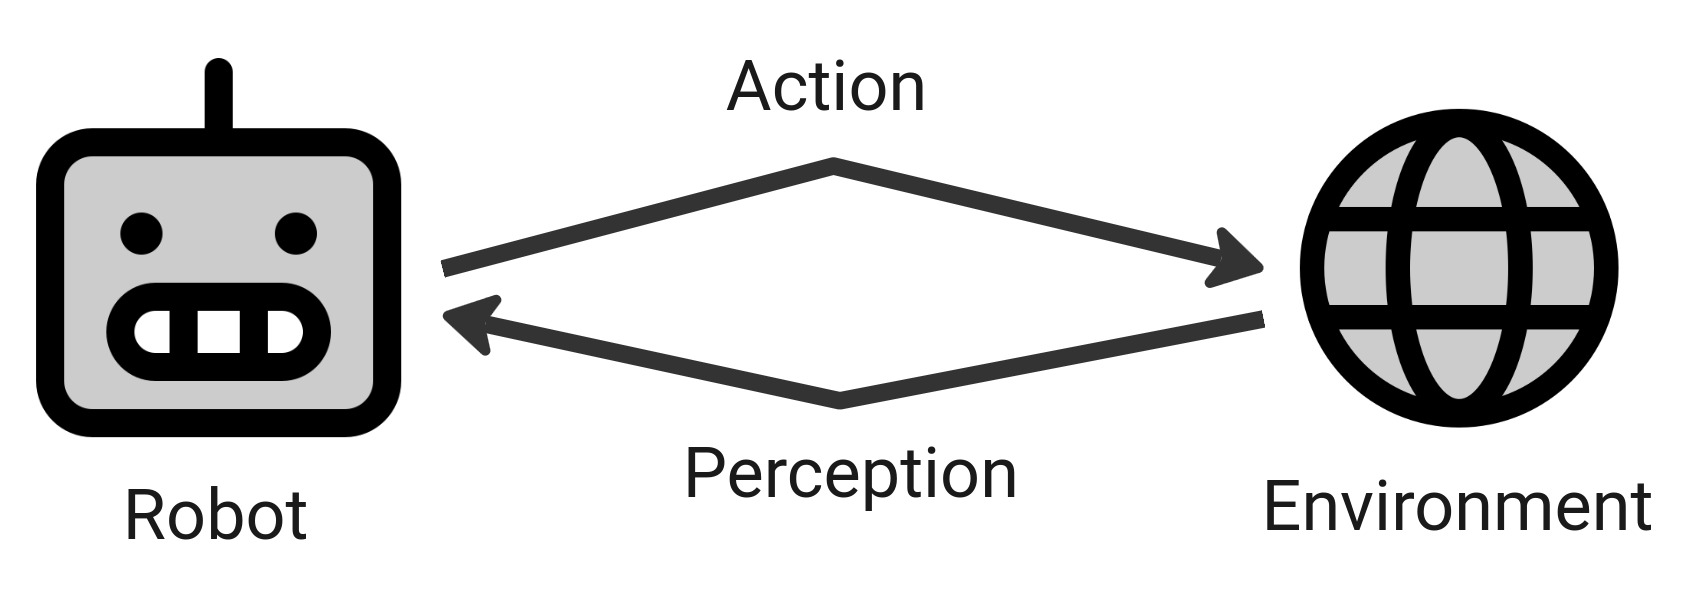
\includegraphics[width=0.7\linewidth]{robot-env.jpg}
    \caption[Perception in the Robot-Environment exchange]{A simplified interpretation of the robotics paradigm. The interaction between an agent and its environment can be seen as a two-way flow: the agent alters the environment through its actions, and uses perception to observe it.}
    \label{fig:robot-env}
\end{figure}

% Just as the human senses span multiple stimulus modalities, so does artificial perception, through the use of different types of sensors. An initial categorization differentiates between proprioceptive and exteroceptive sensors. The first type refers to sensors that provide information about the internal state of the system (virtually independent from the environment), while the second type consists of sensors that collect data about the world. Another division classifies sensors as active (emitting some form of energy in order to obtain a reading) or passive (which simply react to external stimuli).

Sensing modalities have largely different contributions to the perception mechanism. To this extent, the phrase \emph{visual dominance} was introduced by F. Colavita \cite{colavita1974human}, whose study demonstrated that humans focus more on the visual component when presented with an audiovisual stimulus, and following research has strongly confirmed this tendency \cite{Hutmacher2019} \cite{hecht2009sensory}. Unsurprisingly, a similar pattern is emerging in the case of robots, thanks to the reduced cost, familiarity and wide availability of cameras. In many situations, visual stimuli provide most of the necessary information, and this has motivated the development of various image processing algorithms.

Technological innovation in the last century has lead to the situation in which artificial sensors surpass humans in both the range of signals that are perceived, as well as the accuracy of the measurements. A relevant example is the class of \acrfull{lidar} sensors which retrieve three-dimensional information about the environment at a very high frequency and with rather negligible measurement errors, in the form of \emph{\glspl{pointcloud}}. Among many applications, this type of sensors can be used to construct virtual representations of a specific environment, enabling engineers to experiment with a realistic model, evaluate construction progress or validate a finished project.

\section{Problem definition}

The current work addresses a common and well-known problem in the area of \gls{fieldrob}, namely \acrfull{slam}, and combines the practicality of an industrial solution with a perception-based approach.

\begin{figure}
    \centering
    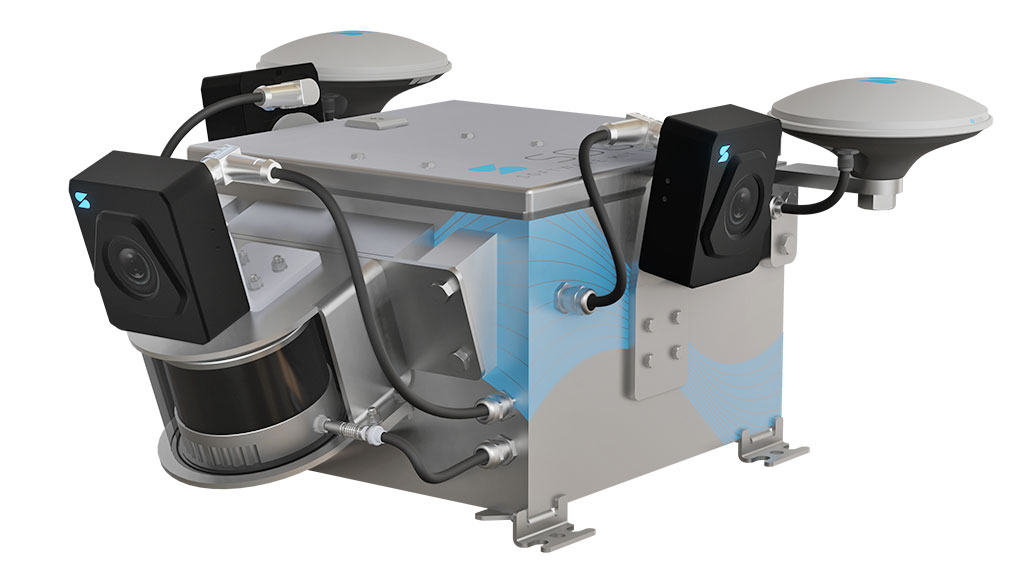
\includegraphics[width=0.6\linewidth]{images/sdx-compact.jpg}
    \caption[SDX-Compact]{The SDX-Compact manufactured by Sodex Innovations GmbH. The set of sensors consists of a 3D LiDAR scanner, three RGB cameras and a high-accuracy positioning system. Image source: \href{https://fieldwork.ch/de/produkte/geopositioning/mobile-datenerfassung/sdx-compact}{Fieldwork}}
    \label{fig:sdx-compact}
\end{figure}

SDX-Compact \reffig{sdx-compact} is the main product of Sodex Innovations GmbH, consisting of multiple sensors that collect spatial and visual data. This module can be easily mounted on an arbitrary vehicle in order to expand its perception capabilities and convert it into a \gls{surveying} device. While the vehicle is moving, the LiDAR sensor captures 3D scans of the surroundings, as well as related metadata (timestamps, localization information, signal intensity etc.). Because the rig includes a high-accuracy \acrfull{ins}, the localization and orientation data can be used to join the collected point clouds and create a global 3D map of the traversed space.

Nonetheless, this suffers from two main limitations:

\begin{compactitem}
    \item Reliance on unstable signal: internally, the  depends on information from a \acrfull{gnss} receiver, which is limited to outdoor spaces and whose availability varies depending on weather conditions and surroundings (e.g. thick vegetation, tall buildings, bridges). 
    \item Unsatisfactory accuracy: when merging point cloud data, positioning or localization errors introduce inconsistencies in the final 3D model, which hinders precise planning and construction.
\end{compactitem}

Our work aims to address these limitations by introducing a component that utilizes the information collected by the LiDAR sensor in conjunction with the existing data. Three research questions have been formulated to guide this process:

\begin{compactenum}
    \item What metrics exist for measuring the accuracy of point cloud \gls{registration}? In this context, registration refers to placing a pair of related point sets in a common reference frame.

    \item Can methods that use only visual information achieve higher quality point cloud registration (3D mapping) than merging based on \acrfull{rtk}? Usually, GNSS systems provide meter-level accuracy. In the current scenario, however, the system is corrected using Real-Time Kinematics, such that the expected error is at centimeter-level.

    \item To what extent is LiDAR-based \gls{odometry} an alternative to GNSS localization? Previous research indicates that the spatial information present in 3D point clouds could be used to compute the relative displacement between consecutive scans, resulting in the ability to estimate odometry (an essential component of robotic localization) without dedicated sensors such as wheel encoders or accelerometers.
\end{compactenum}

The main contribution of the project consists of developing an original framework for localization and mapping based on data collected with an industrial sensor rig. The results are more generic than if a particular physical robotic system were involved, and thus are relevant for virtually any robotic application with a similar setup.

The following chapters of this document will cover related research directions and efforts that our work builds upon \refch{review}, a detailed description of the components and algorithms involved in developing the project \refch{methodology}, an evaluation of the method based on its results \refch{results}, as well as a series of conclusions that were drawn from the overall process \refch{conclusion}.

% evaluation to enable future use
% document structure



% research questions
% motivation/justification
% scope, limitations

\cleardoublepage

\chapter{Literature Review}
\label{ch:review}

The goal of this chapter is to present the research context in which our project was conducted, by looking at common methods for each of the main components and highlighting those that inspired the current approach.

In mobile robotics, map is an important prerequisite that enables robots to operate and perform different tasks such as navigation, obstacle avoidance, path planning, etc. \par \par  
\noindent Simultaneous Localization and Mapping (SLAM) is the most popular method in the literature to generate maps. Among the different methods of SLAM, vision-based and Light Detection and Ranging(LiDAR) technologies are the most popular in the literature. Although each SLAM method has its advantages and drawbacks, they are essential for different tasks. LiDAR technologies will likely remain essential for years to come due to their numerous advantages: robust to various lighting conditions, accurate 3D measurements with higher Field of View (FoV), among others, despite their high cost and bulkiness to install in small-scale robots like drones. Solid-state LiDARs are cost-effective, lightweight, and precise, making them ideal for UAVs in mapping and complex environments. 
\\ \\
Although these solid-state LiDARs have good potential, they have presented new challenges to SLAM solutions: 1) When the robot is operating in a cluttered environment, there not be strong features with geometric shapes like edges and planes. This causes the LiDAR SLAM to degenerate easily. 2) Fusing many feature points with Inertial Measurement Units (IMU) is challenging. 3) LiDAR points are sequentially sampled resulting in each point having a different timestamp which causes motion distortion that severely affects the point registration \cite{xu2021fastlio}.
\\ \\
Several works exist in the literature on LiDAR SLAM. Some of these works use filter-based (Kalman filter) approach while others use optimization-based(factor graphs) for the state estimation. Although filter-based approaches are simple in terms of implementation and computational requirements, they accumulate errors over time causing a larger drift. Optimization-based approaches on the other hand formulate the SLAM problem as non-linear problem and optimize the whole robot trajectory and the map minimizing the drift, more specifically during loop closure. Here we review the most related and relevant works.
\section{Related works}
\cite{zhang2014loam} proposed a real-time method for odometry and mapping. They achieved low-drift results without the need to use IMU and high-accuracy range measurements. The costly SLAM problem is divided into to algorithms where one algorithm computes the odometry at a higher frequency and the other algorithm runs at a much lower frequency to register point cloud.
\\ \\
A method by \cite{xu2021fastlio} presented a novel approach to tightly-coupled LiDAR-inertial odometry by proposing a new formula for computing the Kalman gain, which demonstrates equivalence to the conventional formula but reduces computation complexity based on state dimensions rather than measurement dimensions. An Iterative Kalman Filter(IKF) is used to minimize the point-to-plane distance during the registration of scan to map. The authors implemented their method into a robust LiDAR-inertial odometry package called FAST-LIO that operates effectively on a small-scale quadrotor. Experiments conducted in varied environments validate the system's resilience against fast motion and vibration noise.
\\ \\
\cite{kim2018scan} presented Scan Context, a novel spatial descriptor designed for outdoor place recognition using 3D LiDAR scans. Unlike traditional histogram-based methods, Scan Context encodes the entire point cloud into a matrix format, preserving the absolute geometrical structure of the environment. This approach utilizes a cosine distance measure for similarity scoring and implements a two-phase search algorithm to enhance loop detection efficiency, particularly in urban settings. Experimental results demonstrate that Scan Context significantly outperforms existing global descriptors in various datasets, providing robust performance against noise and viewpoint changes.

\paragraph{}  
\cite{10024300} present a novel approach for large-scale LiDAR mapping by introducing a hierarchical LiDAR bundle adjustment (HLBA) framework. The method aims to improve the consistency and accuracy of LiDAR-based maps by formulating a global optimization problem that jointly refines multiple scans. Unlike conventional SLAM techniques that rely on pairwise constraints, HLBA leverages a hierarchical structure to balance local precision and global consistency, mitigating drift accumulation over extended trajectories. The authors demonstrate the effectiveness of their approach through extensive experiments on real-world datasets, showcasing its advantages in handling large-scale environments with minimal loop closures. Their results indicate that HLBA outperforms existing methods in terms of mapping accuracy and robustness, particularly in scenarios with sparse revisits.

\paragraph{}  
A key contribution of this work is the introduction of an efficient optimization strategy that scales well with the number of LiDAR scans. By organizing the LiDAR data into hierarchical layers, the proposed framework enables efficient refinement without requiring excessive computational resources. The authors also incorporate a robust outlier rejection mechanism to enhance data association, ensuring reliable pose estimation in challenging conditions. Furthermore, the method integrates seamlessly with existing LiDAR-based odometry pipelines, making it adaptable to various robotic platforms. Overall, this study provides a significant advancement in large-scale LiDAR mapping, offering a practical solution for long-term autonomous navigation and high-fidelity 3D reconstruction.


\begin{figure}[h]
	\centering
	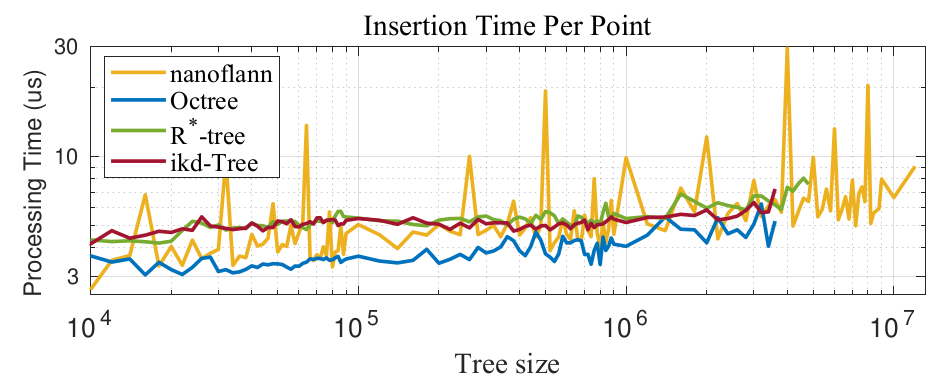
\includegraphics[width=\textwidth]{images/insert.png}
	\caption{ Insertion time per point performance of data structures for map management}
	\label{fig:insertion}
\end{figure}
\begin{figure}[ht!]
	\centering
	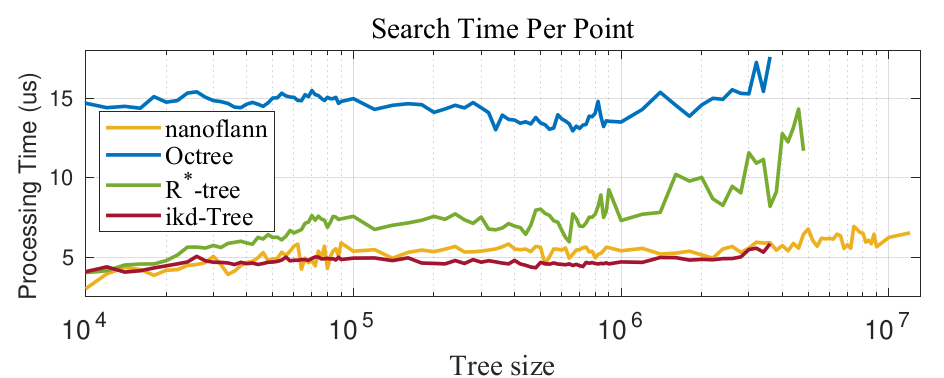
\includegraphics[width=\textwidth]{images/search.png}
	\caption{ Search time per point performance of data structures for map management}
	\label{fig:searching}
\end{figure}

\noindent \cite{xu2022fast} significantly improved upon the original work \cite{xu2021fastlio} by introducing two key advancements: direct point registration and the incremental k-D tree (\textit{ikd-Tree}). Unlike \cite{xu2021fastlio}, which relies on hand-crafted feature extraction, the new approach registers raw LiDAR points directly to the map, increasing accuracy and adaptability to different LiDAR sensors. The newly introduced ikd$\-$Tree enables efficient incremental updates, dynamic re-balancing, and on-tree downsampling, reducing computational load while maintaining real-time performance. These improvements allow a new approach to achieve higher accuracy at a lower computational cost, making it more robust for diverse environments, including those with small FoV LiDARs and aggressive motion.


As showing Figure \ref{fig:insertion} and Figure \ref{fig:searching}, ikd-Tree data structure achieves best overall performance both for point insertion time and point search time.
\cleardoublepage

\chapter{Methodology}
\label{ch:methodology}

% Hardware

% Datasets


% LiDAR

% GNSS

% RTK

\cleardoublepage

\chapter{Results}
\label{ch:results}


% Things worth mentioning
% - execution time
\cleardoublepage

\chapter{Conclusion}
\label{ch:conclusion}

% Future improvements:
% integrate RGB data
% 
\cleardoublepage

% \input{samples_en/intro.tex}
% \cleardoublepage

% \chapter{User documentation}
\label{ch:user}

Lorem ipsum dolor sit amet $\mathbb{N}$\nomenclature{$\mathbb{N}$}{Set of natural numbers}, consectetur adipiscing elit. Duis nibh leo, dapibus in elementum nec, aliquet id sem. Suspendisse potenti. Nullam sit amet consectetur nibh. Donec scelerisque varius turpis at tincidunt. Cras a diam in mauris viverra vehicula. Vivamus mi odio, fermentum vel arcu efficitur, lacinia viverra nibh. Aliquam aliquam ante mi, vel pretium arcu dapibus eu. Nulla finibus ante vel arcu tincidunt, ut consectetur ligula finibus. Mauris mollis lectus sed ipsum bibendum, ac ultrices erat dictum. Suspendisse faucibus euismod lacinia $\mathbb{Z}$\nomenclature{$\mathbb{Z}$}{Set of integer numbers}.


\section{Enumerations and lists}

Etiam vel odio ante. Etiam pulvinar nibh quis massa auctor congue. Pellentesque quis odio vitae sapien molestie vestibulum sit amet et quam. Pellentesque vel dui eget enim hendrerit finibus at sit amet libero. Quisque sollicitudin ultrices enim, nec porta magna imperdiet vitae. Cras condimentum nunc dui, eget molestie nunc accumsan vel.

\begin{itemize}
	\item Fusce in aliquet neque, in pretium sem.
	\item Donec tincidunt tellus id lectus pretium fringilla.
	\item Nunc faucibus, erat pretium tempus tempor, tortor mi fringilla neque, ac congue ex dui vitae mauris.
\end{itemize}

Donec dapibus sodales ante, at scelerisque nunc laoreet sit amet. Mauris porttitor tincidunt neque, vel ullamcorper neque pulvinar et. Integer eu lorem euismod, faucibus lectus sed, accumsan felis. Nunc ornare mi at augue vulputate, eu venenatis magna mollis. Nunc sed posuere dui, et varius nulla. Sed mollis nibh augue, eget scelerisque eros ornare nec.

\begin{enumerate}
	\item\label{step:first} Donec pretium et quam a cursus. Ut sollicitudin tempus urna et mollis.
	\item Aliquam et aliquam turpis, sed fermentum mauris. Nulla eget ex diam.
	\item Donec eget tellus pharetra, semper neque eget, rutrum diam Step~\ref{step:first}.
\end{enumerate}

Praesent porta, metus eget eleifend consequat, eros ligula eleifend ex, a pellentesque mi est vitae urna. Vivamus turpis nunc, iaculis non leo eget, mattis vulputate tellus. Maecenas rutrum eros sem, pharetra interdum nulla porttitor sit amet. In vitae viverra ante. Maecenas sit amet placerat orci, sed tincidunt velit. Vivamus mattis, enim vel suscipit elementum, quam odio venenatis elit\footnote{Phasellus faucibus varius purus, nec tristique enim porta vitae.}, et mollis nulla nunc a risus. Praesent purus magna, tristique sed lacus sit amet, convallis malesuada magna. 

\begin{description}
	\item[Vestibulum venenatis] malesuada enim, ac auctor erat vestibulum et. Phasellus id purus a leo suscipit accumsan.
	\item[Orci varius natoque] penatibus et magnis dis parturient montes, nascetur ridiculus mus. Nullam interdum rhoncus nisl, vel pharetra arcu euismod sagittis. Vestibulum ac turpis auctor, viverra turpis at, tempus tellus.
	\item[Morbi dignissim] erat ut rutrum aliquet. Nulla eu rutrum urna. Integer non urna at mauris scelerisque rutrum sed non turpis.
\end{description}

\subsection{Lists with narrow spacing inbetween items}

Phasellus ultricies, sapien sit amet ultricies placerat, velit purus viverra ligula, id consequat ipsum odio imperdiet enim:
\begin{compactenum}
	\item Maecenas eget lobortis leo.
	\item Donec eget libero enim.
	\item In eu eros a eros lacinia maximus ullamcorper eget augue.
\end{compactenum}

\bigskip

In quis turpis metus. Proin maximus nibh et massa eleifend, a feugiat augue porta. Sed eget est purus. Duis in placerat leo. Donec pharetra eros nec enim convallis:
\begin{compactitem}
	\item Pellentesque odio lacus.
	\item Maximus ut nisl auctor.
	\item Sagittis vulputate lorem.
\end{compactitem}

\bigskip

Vestibulum ante ipsum primis in faucibus orci luctus et ultrices posuere cubilia Curae; Sed lorem libero, dignissim vitae gravida a, ornare vitae est.
\begin{compactdesc}
	\item[Cras maximus] massa commodo pellentesque viverra.
	\item[Morbi sit] amet ante risus. Aliquam nec sollicitudin mauris
	\item[Ut aliquam rhoncus sapien] luctus viverra arcu iaculis posuere
\end{compactdesc}


\section{Images and figures}

Aliquam vehicula luctus mi a pretium. Nulla quam neque, maximus nec velit in, aliquam mollis tortor. Aliquam erat volutpat. Curabitur vitae laoreet turpis. Integer id diam ligula. Nulla sodales purus id mi consequat, eu venenatis odio pharetra. Cras a arcu quam. Suspendisse augue risus, pulvinar a turpis et, commodo aliquet turpis. Nulla aliquam scelerisque mi eget pharetra. Mauris sed posuere elit, ac lobortis metus. Proin lacinia sit amet diam sed auctor. Nam viverra orci id sapien sollicitudin, a aliquam lacus suscipit, Figure~\ref{fig:example-1}:

\begin{figure}[H]
	\centering
	
\includegraphics[width=0.6\textwidth,height=100px]{elte_cimer_szines}
	\caption{Quisque ac tincidunt leo}
	\label{fig:example-1}
\end{figure}

\subsection{Framing figures}

Ut aliquet nec neque eget fermentum. Cras volutpat tellus sed placerat elementum. Quisque neque dui, consectetur nec finibus eget, blandit id purus. Nam eget ipsum non nunc placerat interdum.

\begin{figure}[H]
	\centering
	
\includegraphics[width=0.6\textwidth,height=100px,frame]{elte_cimer_szines}
	\caption{Quisque ac tincidunt leo}
\end{figure}

\subsection{Subfigures}

In non ipsum fermentum urna feugiat rutrum a at odio. Pellentesque habitant morbi tristique senectus et netus et malesuada fames ac turpis egestas. Nulla tincidunt mattis nisl id suscipit. Sed bibendum ac felis sed volutpat. Nam pharetra nisi nec facilisis faucibus. Aenean tristique nec libero non commodo. Nulla egestas laoreet tempus. Nunc eu aliquet nulla, quis vehicula dui. Proin ac risus sodales, gravida nisi vitae, efficitur neque, Figure~\ref{fig:example-2}:

\begin{figure}[H]
	\centering
	\subcaptionbox{Vestibulum quis mattis urna}{
		
\includegraphics[width=0.45\linewidth]{elte_cimer_szines}}
	\hspace{5pt}
	\subcaptionbox{Donec hendrerit quis dui sit amet venenatis}{
		
\includegraphics[width=0.45\linewidth]{elte_cimer_szines}}
	\caption{Aenean porttitor mi volutpat massa gravida}
	\label{fig:example-2}
\end{figure}

Nam et nunc eget elit tincidunt sollicitudin. Quisque ligula ipsum, tempor vitae tortor ut, commodo rhoncus diam. Pellentesque habitant morbi tristique senectus et netus et malesuada fames ac turpis egestas. Phasellus vehicula quam dui, eu convallis metus porta ac.


\section{Tables}

Nam magna ex, euismod nec interdum sed, sagittis nec leo. Nam blandit massa bibendum mattis tristique. Phasellus tortor ligula, sodales a consectetur vitae, placerat vitae dolor. Aenean consequat in quam ac mollis. 

\begin{table}[H]
	\centering
	\begin{tabular}{ | m{0.25\textwidth} | m{0.65\textwidth} | }
		\hline
		\textbf{Phasellus tortor} & \textbf{Aenean consequat} \\
		\hline \hline
		\emph{Sed malesuada} & Aliquam aliquam velit in convallis ultrices. \\
		\hline
		\emph{Purus sagittis} &  Quisque lobortis eros vitae urna lacinia euismod. \\
		\hline
		\emph{Pellentesque} & Curabitur ac lacus pellentesque, eleifend sem ut, placerat enim. Ut auctor tempor odio ut dapibus. \\
		\hline
	\end{tabular}
	\caption{Maecenas tincidunt non justo quis accumsan}
	\label{tab:example-1}
\end{table}

\subsection{Multi rows and multi columns}

Mauris a dapibus lectus. Vestibulum commodo nibh ante, ut maximus magna eleifend vel. Integer vehicula elit non lacus lacinia, vitae porttitor dolor ultrices. Vivamus gravida faucibus efficitur. Ut non erat quis arcu vehicula lacinia. Nulla felis mauris, laoreet sed malesuada in, euismod et lacus. Aenean at finibus ipsum. Pellentesque dignissim elit sit amet lacus congue vulputate.

\begin{table}[htb]
	\centering
	\begin{tabular}{ | c | r | r | r | r | r | r | }
		\hline
		\multirow{2}{*}{\textbf{Quisque}} & \multicolumn{2}{ c | }{\textbf{Suspendisse}} & \multicolumn{2}{ c | }{\textbf{Aliquam}} & \multicolumn{2}{ c | }{\textbf{Vivamus}} \\
		\cline{2-7}
		& Proin & Nunc & Proin & Nunc & Proin & Nunc \\
		\hline \hline		
		Leo & 2,80 MB & 100\% & 232 KB & 8,09\% & 248 KB & 8,64\% \\
		\hline
		Vel & 9,60 MB & 100\% & 564 KB & 5,74\% & 292 KB & 2,97\% \\
		\hline
		Auge & 78,2 MB & 100\% & 52,3 MB & 66,88\% & 3,22 MB & 4,12\% \\
		\hline 
	\end{tabular}
	\caption[Rövid cím a táblázatjegyzékbe]{Vivamus ac arcu fringilla, fermentum neque sed, interdum erat. Mauris bibendum mauris vitae enim mollis, et eleifend turpis aliquet.}
	\label{tab:example-2}
\end{table}

\subsection{Long tables over multiple pages}

Nunc porta placerat leo, sit amet porttitor dui porta molestie. Aliquam at fermentum mi. Maecenas vitae lorem at leo tincidunt volutpat at nec tortor. Vivamus semper lacus eu diam laoreet congue. Vivamus in ipsum risus. Nulla ullamcorper finibus mauris non aliquet. Vivamus elementum rhoncus ex ut porttitor.

\begin{center}
	\begin{longtable}{ | p{0.3\textwidth} | p{0.7\textwidth} | }
		
		\hline
		\multicolumn{2}{|c|}{\textbf{Praesent aliquam mauris enim}}
		\\ \hline
		
		\emph{Suspendisse potenti} & \emph{Lorem ipsum dolor sit amet}
		\\ \hline \hline
		\endfirsthead % table header on first page
		
		\hline
		\emph{Suspendisse potenti} & \emph{Lorem ipsum dolor sit amet}
		\\ \hline \hline
		\endhead % table header on further pages
		
		\hline
		\endfoot % table footer on previous pages
		
		\endlastfoot % table footer on last page
		
		\emph{Praesent}
		& Nulla ultrices et libero sit amet fringilla. Nunc scelerisque ante tempus sapien placerat convallis.
		\\ \hline
		
		\emph{Luctus}
		& Integer hendrerit erat massa, non hendrerit risus convallis at. Curabitur ultrices, justo in imperdiet condimentum, neque tortor luctus enim, luctus posuere massa erat vitae nibh.
		\\ \hline
		
		\emph{Egestas}
		& Duis fermentum feugiat augue in blandit. Mauris a tempor felis. Pellentesque ultricies tristique dignissim. Pellentesque aliquam semper tristique. Nam nec egestas dolor. Vestibulum id elit quis enim fringilla tempor eu a mauris. Aliquam vitae lacus tellus. Phasellus mauris lectus, aliquam id leo eget, auctor dapibus magna. Fusce lacinia felis ac elit luctus luctus.
		\\ \hline
		
		\emph{Dignissim}
		& Praesent aliquam mauris enim, vestibulum posuere massa facilisis in. Suspendisse potenti. Nam quam purus, rutrum eu augue ut, varius vehicula tellus. Fusce dui diam, aliquet sit amet eros at, sollicitudin facilisis quam. Phasellus tempor metus vel augue gravida pretium. Proin aliquam aliquam blandit. Nulla id tempus mi. Fusce in aliquam tortor.
		\\ \hline
		
		\emph{Pellentesque}
		& Donec felis nibh, imperdiet a arcu non, vehicula gravida nibh. Quisque interdum sapien eu massa commodo, ac elementum felis faucibus.
		\\ \hline
		
		\emph{Molestie}
		& Cras ullamcorper tellus et auctor ultricies. Maecenas tincidunt euismod lectus nec venenatis. Suspendisse potenti. Pellentesque pretium nunc ut euismod cursus. Nam venenatis condimentum quam. Curabitur suscipit efficitur aliquet. Interdum et malesuada fames ac ante ipsum primis in faucibus.
		\\ \hline
		
		\emph{Vivamus semper}
		& In purus purus, faucibus eu libero vulputate, tristique sodales nunc. Nulla ut gravida dolor. Fusce vel pellentesque mi, vel efficitur eros. Nunc vitae elit tellus. Sed vestibulum auctor consequat. 
		\\ \hline
		
		\emph{Condimentum}
		& Nulla scelerisque, leo et facilisis pretium, risus enim cursus turpis, eu suscipit ipsum ipsum in mauris. Praesent eget pulvinar ipsum, suscipit interdum nunc. Nam varius massa ut justo ullamcorper sollicitudin. Vivamus facilisis suscipit neque, eu fermentum risus. Ut at mi mauris.
		\\ \hline
		
		\caption{Praesent ullamcorper consequat tellus ut eleifend}
		\label{tab:example-3}		
	\end{longtable}
\end{center}
% \cleardoublepage

% \chapter{Developer documentation}
\label{ch:impl}

Lorem ipsum dolor sit amet, consectetur adipiscing elit. Duis nibh leo, dapibus in elementum nec, aliquet id sem. Suspendisse potenti. Nullam sit amet consectetur nibh. Donec scelerisque varius turpis at tincidunt.


\section{Theorem-like environments}

\begin{definition}
Mauris tristique sollicitudin ultrices. Etiam tristique quam sit amet metus dictum imperdiet. Nunc id lorem sed nisl pulvinar aliquet vitae quis arcu. Morbi iaculis eleifend porttitor.
\end{definition}

Maecenas rutrum eros sem, pharetra interdum nulla porttitor sit amet. In vitae viverra ante. Maecenas sit amet placerat orci, sed tincidunt velit. Vivamus mattis, enim vel suscipit elementum, quam odio venenatis elit, et mollis nulla nunc a risus. Praesent purus magna, tristique sed lacus sit amet, convallis malesuada magna. Phasellus faucibus varius purus, nec tristique enim porta vitae.

\begin{theorem}
Nulla finibus ante vel arcu tincidunt, ut consectetur ligula finibus. Mauris mollis lectus sed ipsum bibendum, ac ultrices erat dictum. Suspendisse faucibus euismod lacinia. Etiam vel odio ante.
\end{theorem}
\begin{proof}
Etiam pulvinar nibh quis massa auctor congue. Pellentesque quis odio vitae sapien molestie vestibulum sit amet et quam. Pellentesque vel dui eget enim hendrerit finibus at sit amet libero. Quisque sollicitudin ultrices enim, nec porta magna imperdiet vitae. Cras condimentum nunc dui.
\end{proof}

Donec dapibus sodales ante, at scelerisque nunc laoreet sit amet. Mauris porttitor tincidunt neque, vel ullamcorper neque pulvinar et. Integer eu lorem euismod, faucibus lectus sed, accumsan felis. 

\begin{remark}
Nunc ornare mi at augue vulputate, eu venenatis magna mollis. Nunc sed posuere dui, et varius nulla. Sed mollis nibh augue, eget scelerisque eros ornare nec. Praesent porta, metus eget eleifend consequat, eros ligula eleifend ex, a pellentesque mi est vitae urna. Vivamus turpis nunc, iaculis non leo eget, mattis vulputate tellus.
\end{remark}

Fusce in aliquet neque, in pretium sem. Donec tincidunt tellus id lectus pretium fringilla. Nunc faucibus, erat pretium tempus tempor, tortor mi fringilla neque, ac congue ex dui vitae mauris. Donec pretium et quam a cursus.

\begin{note}
Aliquam vehicula luctus mi a pretium. Nulla quam neque, maximus nec velit in, aliquam mollis tortor. Aliquam erat volutpat. Curabitur vitae laoreet turpis. Integer id diam ligula.
\end{note}

Ut sollicitudin tempus urna et mollis. Aliquam et aliquam turpis, sed fermentum mauris. Nulla eget ex diam. Donec eget tellus pharetra, semper neque eget, rutrum diam.

\subsection{Equations, formulas}

Duis suscipit ipsum nec urna blandit, $2 + 2 = 4$ pellentesque vehicula quam fringilla. Vivamus euismod, lectus sit amet euismod viverra, dolor metus consequat sapien, ut hendrerit nisl nulla id nisi. Nam in leo eu quam sollicitudin semper a quis velit.

$$a^2 + b^2 = c^2$$

Phasellus mollis, elit sed convallis feugiat, dolor quam dapibus nibh, suscipit consectetur lacus risus quis sem. Vivamus scelerisque porta odio, vitae euismod dolor accumsan ut.

In mathematica, identitatem Euleri (equation est scriptor vti etiam notum) sit aequalitatem Equation~\ref{eq:euler}:
\begin{equation}\label{eq:euler}
e^{i \times \pi} + 1 = 0
\end{equation}

Vestibulum ante ipsum primis in faucibus orci luctus et ultrices posuere cubilia curae; Nullam pulvinar purus at pharetra elementum.
Aequationes adsignans aequationis signum:
\begin{align}
	A & = \frac{\pi r^2}{2} \\
	& = \frac{1}{2} \pi r^2
\end{align}

Proin tempor risus a efficitur condimentum. Cras lobortis ligula non sollicitudin euismod. Fusce non pellentesque nibh, non elementum tellus.
Omissa numeratione aliquarum aequationum:
\begin{align}
	f(u) & =\sum_{j=1}^{n} x_jf(u_j) \nonumber \\
	& =\sum_{j=1}^{n} x_j \sum_{i=1}^{m} a_{ij}v_i \nonumber \\
	& =\sum_{j=1}^{n} \sum_{i=1}^{m} a_{ij}x_jv_i
\end{align}

\section{Source code samples}

Nulla sodales purus id mi consequat, eu venenatis odio pharetra. Cras a arcu quam. Suspendisse augue risus, pulvinar a turpis et, commodo aliquet turpis. Nulla aliquam scelerisque mi eget pharetra. Mauris sed posuere elit, ac lobortis metus. Proin lacinia sit amet diam sed auctor. Nam viverra orci id sapien sollicitudin, a aliquam lacus suscipit. Quisque ac tincidunt leo Code~\ref{src:cpp} and \ref{src:csharp}:

\lstset{caption={Hello World in C++}, label=src:cpp}
\begin{lstlisting}[language={C++}]
#include <stdio>

int main() 
{
	int c;
	std::cout << "Hello World!" << std::endl;

	std::cout << "Press any key to exit." << std::endl;
	std::cin >> c;
	
	return 0;
}
\end{lstlisting}

\lstset{caption={Hello World in C\#}, label=src:csharp}
\begin{lstlisting}[language={[Sharp]C}]
using System;
namespace HelloWorld
{
	class Hello 
	{
		static void Main() 
		{
			Console.WriteLine("Hello World!");
			
			Console.WriteLine("Press any key to exit.");
			Console.ReadKey();
		}
	}
}
\end{lstlisting}

\subsection{Algorithms}

A general Interval Branch and Bound algorithm is shown in Algorithm~\ref{alg:ibb}. An appropriate selection rule is applied in Step~\ref{step:selrule}.\\
Source of example: \href{https://www.inf.u-szeged.hu/actacybernetica/}{Acta Cybernetica (this is a hyperlink)}.

\begin{algorithm}[H]
\caption{A general interval B\&B algorithm} 
\label{alg:ibb} 
\textbf{\underline{Funct}} IBB($S,f$)
\begin{algorithmic}[1] % display line numbers before every n line, here n = 1
\State Set the working list ${\cal L}_W$ := $\{S\}$ and the final list ${\cal L}_Q$ := $\{\}$     
\While{( ${\cal L}_W \neq \emptyset$ )} \label{alg:igoend}
	\State  Select an interval $X$ from ${\cal L}_W$ \label{step:selrule}\Comment{Selection rule}  
	\State Compute $lbf(X)$ \Comment{Bounding rule}		  
	\If{$X$ cannot be eliminated} \Comment{Elimination rule}
		\State Divide $X$ into $X^j,\ j=1,\dots, p$, subintervals   \Comment{Division rule}
		\For{$j=1,\ldots,p$}
			\If{$X^j$ satisfies the termination criterion} \Comment{Termination rule}
				\State Store $X^j$ in ${\cal L}_W$ 
			\Else
				\State Store $X^j$ in ${\cal L}_W$ 
			\EndIf
		\EndFor  
	\EndIf
\EndWhile
\State \textbf{return} ${\cal L}_Q$
\end{algorithmic}
\end{algorithm}

% \cleardoublepage

% \input{samples_en/sum.tex}
% \cleardoublepage

% Acknowledgements (optional) - in case your thesis received funding or would like to express special thanks to someone
% \chapter*{\acklabel}
% \addcontentsline{toc}{chapter}{\acklabel}
% In case your thesis received financial support from a project or the university, it is usually required to indicate the proper attribution in the thesis itself. Special thanks can also be expressed towards teachers, fellow students and colleagues who helped you in the process of creating your thesis.

% Appendices (optional) - useful for detailed information in long tables, many and/or large figures, etc.
% \appendix
% \chapter{Simulation results}
\label{appx:simulation}

Lorem ipsum dolor sit amet, consectetur adipiscing elit. Pellentesque facilisis in nibh auctor molestie. Donec porta tortor mauris. Cras in lacus in purus ultricies blandit. Proin dolor erat, pulvinar posuere orci ac, eleifend ultrices libero. Donec elementum et elit a ullamcorper. Nunc tincidunt, lorem et consectetur tincidunt, ante sapien scelerisque neque, eu bibendum felis augue non est. Maecenas nibh arcu, ultrices et libero id, egestas tempus mauris. Etiam iaculis dui nec augue venenatis, fermentum posuere justo congue. Nullam sit amet porttitor sem, at porttitor augue. Proin bibendum justo at ornare efficitur. Donec tempor turpis ligula, vitae viverra felis finibus eu. Curabitur sed libero ac urna condimentum gravida. Donec tincidunt neque sit amet neque luctus auctor vel eget tortor. Integer dignissim, urna ut lobortis volutpat, justo nunc convallis diam, sit amet vulputate erat eros eu velit. Mauris porttitor dictum ante, commodo facilisis ex suscipit sed.

Sed egestas dapibus nisl, vitae fringilla justo. Donec eget condimentum lectus, molestie mattis nunc. Nulla ac faucibus dui. Nullam a congue erat. Ut accumsan sed sapien quis porttitor. Ut pellentesque, est ac posuere pulvinar, tortor mauris fermentum nulla, sit amet fringilla sapien sapien quis velit. Integer accumsan placerat lorem, eu aliquam urna consectetur eget. In ligula orci, dignissim sed consequat ac, porta at metus. Phasellus ipsum tellus, molestie ut lacus tempus, rutrum convallis elit. Suspendisse arcu orci, luctus vitae ultricies quis, bibendum sed elit. Vivamus at sem maximus leo placerat gravida semper vel mi. Etiam hendrerit sed massa ut lacinia. Morbi varius libero odio, sit amet auctor nunc interdum sit amet.

Aenean non mauris accumsan, rutrum nisi non, porttitor enim. Maecenas vel tortor ex. Proin vulputate tellus luctus egestas fermentum. In nec lobortis risus, sit amet tincidunt purus. Nam id turpis venenatis, vehicula nisl sed, ultricies nibh. Suspendisse in libero nec nisi tempor vestibulum. Integer eu dui congue enim venenatis lobortis. Donec sed elementum nunc. Nulla facilisi. Maecenas cursus id lorem et finibus. Sed fermentum molestie erat, nec tempor lorem facilisis cursus. In vel nulla id orci fringilla facilisis. Cras non bibendum odio, ac vestibulum ex. Donec turpis urna, tincidunt ut mi eu, finibus facilisis lorem. Praesent posuere nisl nec dui accumsan, sed interdum odio malesuada.
% \cleardoublepage


% Bibliography (mandatory)
\phantomsection
\addcontentsline{toc}{chapter}{\biblabel}
\printbibliography[title=\biblabel]
\cleardoublepage

% List of figures (optional) - useful over 3-5 figures
\phantomsection
\addcontentsline{toc}{chapter}{\lstfigurelabel}
\listoffigures
\cleardoublepage

% List of tables (optional) - useful over 3-5 tables
% \phantomsection
% \addcontentsline{toc}{chapter}{\lsttablelabel}
% \listoftables
% \cleardoublepage

% List of algorithms (optional) - useful over 3-5 algorithms
% \phantomsection
% \addcontentsline{toc}{chapter}{\lstalgorithmlabel}
% \listofalgorithms
% \cleardoublepage

% List of codes (optional) - useful over 3-5 code samples
% \phantomsection
% \addcontentsline{toc}{chapter}{\lstcodelabel}
% \lstlistoflistings
% \cleardoublepage

% List of symbols (optional)
%\printnomenclature

{\setlength{\baselineskip}{0.6\baselineskip} % Adjust 0.9 to reduce spacing
    \printglossary[type=\acronymtype]
    \printglossary
}

\end{document}
